\documentclass{mc2015}

%%%%%%%%%%%%%%%%%%%%%%%%%%%%%%%%%%%%%%%%%%%%%%%%%%%%%%%%%%%%%%%%%%%%%
\usepackage[T1]{fontenc}         % Use T1 encoding instead of OT1
\usepackage[utf8]{inputenc}      % Use UTF8 input encoding
\usepackage{microtype}           % Improve typography
\usepackage{booktabs}            % Publication quality tables
\usepackage{amsmath}
\usepackage{mhchem}
\usepackage{graphicx}
\usepackage{gensymb}
\usepackage{float}
\usepackage{subcaption}
\usepackage[exponent-product=\cdot]{siunitx}
\usepackage[colorlinks,breaklinks]{hyperref}
\hypersetup{linkcolor=black, citecolor=black, urlcolor=black}

\usepackage{lipsum}

\def\equationautorefname{Eq.}
\def\figureautorefname{Fig.}

%%%%%%%%%%%%%%%%%%%%%%%%%%%%%%%%%%%%%%%%%%%%%%%%%%%%%%%%%%%%%%%%%%%%%
% Insert authors' names and short version of title in lines below

\authorHead{Madicken Munk, Leah Morgan, Brett Davidheiser-Kroll, et. al.}
\shortTitle{Design of a Compact Neutron Source for Geochronology Applications}

%%%%%%%%%%%%%%%%%%%%%%%%%%%%%%%%%%%%%%%%%%%%%%%%%%%%%%%%%%%%%%%%%%%%%
\begin{document}

\title{Design and Feasibility Study of a Compact Neutron Source for Extra-terrestrial Geochronology Applications}

\author{Madicken Munk}
\author{Rachel Slaybaugh}
\author{Karl Van Bibber}
\affil{Department of Nuclear Engineering \\
  University of California, Berkeley
  3115B Etcheverry Hall, Berkeley, CA \\
  madicken@berkeley.edu}

\author{Leah Morgan}
\author{Brett Davidheiser-Kroll}
\author{Darren Mark}
\author{Sanjeev Gupta}
\author{Patrick Harkness}
\affil{
  Scottish Universities Environmental Research Centre \\
  Rankine Avenue, East Kilbride G75 0QF, UK \\
  leah.morgan@glasgow.ac.uk
}

\maketitle

\begin{abstract}
The \ce{^{40}Ar}/\ce{^{39}Ar} radiometric dating technique is an attractive option for future martian age-dating applications. However, in-situ \ce{^{40}Ar}/\ce{^{39}Ar} radiometric dating on Mars presents unique challenges to the design of a device capable of achieving sufficient precision on geological samples obtained on the Martian surface. For this application, a fast neutron source with a low thermal neutron flux is ideal for inducing the \ce{^{39}K}(n,p)\ce{^{39}Ar} reaction with few competing reactions that require age-correction factors. This paper explores the design of a neutron emitting device specifically for in-situ geochronological applications on Mars. We have determined that the most feasible design is likely a \ce{^{252}Cf} spontaneous fission source shielded by polyethylene layered with a strong thermal neutron absorber. Although boosting options--induced fission sources, ($\alpha$,n)--are available, they do not provide sufficient neutron multiplicity to justify the increased mass of the device. Furthermore, shielding the rover from the neutron source will likely comprise the largest fractional mass of the device, which will be reduced by shielding only a small solid angle of the source. While we have determined that it is possible to design such a neutron source, there will also be other instrumentation competing for a mass fraction of the Rover instrument payload, which may make it difficult to design a device that achieves the required mass and fluence limitations for a future mission. This work provides an initial path forward in determining a workable design.  

\emph{Key Words}: Fisson Sources, Argon/Argon Geochronology, Mars
\end{abstract}

%%%%%%%%%%%%%%%%%%%%%%%%%%%%%%%%%%%%%%%%%%%%%%%%%%%%%%%%%%%%%%%%%%%%%
\section{Introduction}

One of the goals of the future rover missions includes determining the age of Mars. Recent efforts have been focused on using the \ce{^{40}K}/\ce{^{40}Ar} method \cite{farley_situ_2014,farley_double-spike_2013,cassata_situ_2014} (henceforth referred to as the K/Ar method), with the Curiosity Rover taking measurements with this method. However, there is no sure way to determine if the samples measured underwent a thermal event that would change the calculation of the age because of the way the K/Ar method works. Conversely, the \ce{^{40}Ar}/\ce{^{39}Ar} method \cite{mcdougall_geochronology_1999} (henceforth referred to as Ar/Ar) offers more information on the history of the rock as well as a more reliable age. Furthermore, the benefits of K/Ar dating--the abundance of potassium in geologic samples, the reliability of the method over a large age spectrum--are also present in the Ar/Ar method. The Ar/Ar method has been proposed for extra-terrestrial applications \cite{li_evaluation_2011} in the past, but there has not been extensive work on the feasibility or design of a device capable of supplying the necessities for the Ar/Ar method.

Following the Background Section describing the details of the dating methods, this paper will discuss the design considerations for a neutron-emitting device to irradiate samples for Ar/Ar geochronology applications. Section \ref{sec:design} covers the constraints and details of the device design. The feasibility of device configurations is discussed in Section \ref{sec:feasibility}. Finally, concluding remarks are made in Section \ref{sec:conclusions}. While the authors have considered a number of design configurations for this device, no finalized design is proposed. Rather, this paper is intended to provide a starting point for future designs of Ar/Ar-specific instrumentation on extra-terrestrial missions. 

\section{Background}
The \ce{^{40}K}/\ce{^{40}Ar} method has been widely used, but has some drawbacks. The K/Ar method relies upon the fact that \ce{^{40}K} decays to \ce{^{40}Ar}. Assuming that at the time of formation there is no argon in the sample (a good assumption, as the gas is thermodynamically driven to diffuse out of the molten rock), an age can be calculated with this parent-daughter ratio \cite{mcdougall_geochronology_1999}. However, there are issues that challenge the accuracy of this method. To count the relative abundances of \ce{^{40}K} and \ce{^{40}Ar}, separate processes are required to isolate each element, so two samples are required. Additionally, the abundance counts for each element are an average across each grain forming the macroscopic rock structure. Should some high temperature event occur after formation, migration of the \ce{^{40}Ar} near the grain boundaries can be driven from the rock by temperature-enhanced diffusion. This premature loss of \ce{^{40}Ar} in the sample would skew the parent-daughter age determined from the K/Ar method, thus resulting in an unreliable age that is some value between the formation age and the thermal event. If the rock is heated to a temperature high enough to liberate all of the accrued radiogenic \ce{^{40}Ar}, the calculated K/Ar age will be that of the thermal event, not the formation age. 

An alternative approach to the \ce{^{40}K}/\ce{^{40}Ar} method is the \ce{^{40}Ar}/\ce{^{39}Ar} method. This approach has roots in the K/Ar method, but uses \ce{^{39}Ar} as a proxy for potassium, whereby the \ce{^{39}K}(n,p)\ce{^{39}Ar} reaction is used to generate \ce{^{39}Ar} in the sample. With knowledge of the cross section for the (n,p) reaction and the neutron flux, a reaction rate can be calculated to determine the original \ce{^{39}K} abundance in the sample. Assuming the \ce{^{39}K}/\ce{^{40}K} is constant in nature, the counted \ce{^{39}Ar} abundance can be related to the \ce{^{40}K} abundance in the sample. The age of the sample can then be calculated with the same decay principles as the K/Ar method. Traditionally, this reaction has been induced with neutrons produced by research reactors. An additional sample with a known age is also placed in the irradiation sample chamber and is used to back-calculate the reaction rate for the (n,p) reaction. 

While the Ar/Ar method is essentially a variant of the K/Ar method, it provides a number of advantages over its predecessor. By transmuting the \ce{^{39}K} into \ce{^{39}Ar}, the measurement can be performed on a single element, and eliminates the need for separate samples. Furthermore, as the argon is liberated from the sample (usually by incrementally heating the sample), the changing ratio of \ce{^{40}Ar}/\ce{^{39}Ar} can reveal information about the distribution of K and Ar within the mineral phase. If the sample has no thermal history, the ratio of \ce{^{40}Ar}/\ce{^{39}Ar} should remain constant throughout the sample heating. If there is a thermal history, the distribution of \ce{^{40}Ar}/\ce{^{39}Ar} throughout the sample can reveal both the formation age of the sample and the thermal event. On an extra-terrestrial surface where impact events are commonplace, a thermal event is likely to have affected any sample collected, making Ar/Ar the preferred method. The challenge to using this in practice is taking a device to marks that can induce the \ce{^{39}K}(n,p)\ce{^{39}Ar} reaction.

%%%%%%%%%%%%%%%%%%%%%%%%%%%%%%%%%%%%%%%%%%%%%%%%%%%%%%%%%%%%%%%%%%%%%
\section{Device Design}
\label{sec:design}

The most basic device used for sample irradiation in Ar/Ar geochronology must have (1) a neutron source, (2) a sample chamber, and (3) a neutron shield. To perform Ar/Ar geochronology, additional instrumentation--such as a mass spectrometer and drilling mechanism--is also required. For the purposes of this paper, the neutron emitting device is comprised of the three aforementioned components. The various options that one could use to construct such a device are explored herein. 

The foundation of Ar/Ar geochronology relies upon the transmutation reaction \ce{^{39}K}(n,p)\ce{^{39}Ar}, which cannot be induced without a neutron source. This is the single most important component for the device described in the forthcoming pages. First, the \ce{^{39}K}(n,p)\ce{^{39}Ar} reaction is a threshold reaction, and requires the flux to have some population of fast neutrons to produce \ce{^{39}Ar} in acceptable quantities. However, thermal neutrons also induce competing reactions that make it more difficult to calculate the age \cite{mcdougall_geochronology_1999}, so a device supplying a neutron energy spectrum with a high proportion of fast neutrons is desirable. Second, the neutron source must produce enough \ce{^{39}Ar} that the ratio between \ce{^{40}Ar} and \ce{^{39}Ar} is detectable. Counting the \ce{^{40}Ar}/\ce{^{39}Ar} ratio is limited by the precision of the mass spectrometer that will be available on the rover and by the irradiation time. To achieve a \ce{^{40}Ar}/\ce{^{39}Ar} ratio of $10^{5}:1$ in 100 days, the fast flux requirement is $3.3\times10^9$ n/cm$^2$s. Lastly, the source must have some degree of longevity to last for the rover lifetime. This requires that the neutron source have a long enough half-life or fuel supply to survive the trip to mars and the mission lifetime, while also meeting the fast neutron fluence requirement in $\sim$200 days or less.   

The sample chamber has fewer design limitations than the neutron source. It should have locations to contain the samples, and the neutron energy spectrum should not be perturbed significantly between various sample locations. If the spectrum is perturbed significantly, determining the reaction rate of the \ce{^{39}K}(n,p)\ce{^{39}Ar} transmutation will be required for each sample separately, which will make the Ar/Ar method unnecessarily complex. These goals can be achieved with a small sample chamber constructed out of a metal with a low activation cross section and a poor scattering ratio, like aluminum. The samples must also be easily accessible such that sample handling is feasible. Additionally, both the K/Ar and Ar/Ar methods rely upon the fact that the radiogenic \ce{^{40}Ar} is not lost during sample preparation. Premature loss of accrued Ar in the sample is usually caused by heat-driven diffusion. For the purposes of this device, it must be assured that the sample is not heated above 200\celsius\ during sample preparation or irradiation \cite{mcdougall_geochronology_1999}. This is feasible by designing the device to use a neutron source with a low heat output or with a heat removal system. 
% It just occurred to me: will the source be removable for when you're doing irradiation, or will the irradiation chamber be inside the shield? It might be worth adding a sentence addressing this.

The shield has a variety of restrictions to consider in its design. Even with a low heat output source, the sample chamber may be heated if surrounded by a thermal insulator--which impacts decisions about the materials and the geometric configuration of the shield. The shield must also prioritize protecting the numerous electronic components on the mars rover from neutron damage. The image sensors on Curiosity were radiation hardened up to  $10^{7}$ n/cm$^2$s, which provides a starting point for the flux limits for future rover missions. Furthermore, the rover is limited in the total mass that it is able to carry. The total instrument payload on Curiosity is $\sim$75kg, and the radioisotope thermal generator (RTG) is an additional 45kg. Assuming that future missions will have similar limitations to those currently underway, this can provide an order of magnitude mass limitation for the future mission with the neutron emitting device. This mass requirement inherently limits the total amount of shielding and source material that can be used, and the interplay between what shielding and source material are selected will influence the overall geometry of the device. 

Several geometries that initially appeared to satisfy these requirements were proposed; Fig.\ \ref{fig:geometries} illustrates a few. The first design (Fig.\ \ref{fig:geometries}a), a small point-source with a sample chamber surrounded by a large spherical shield, was proposed to maximize shield thickness and ideally protect both the martian surface and the mars rover from neutron damage. The success of this design is contingent upon finding a low mass, low volume source that can be surrounded by a sample chamber. It also requires that the shield does not thermally insulate the sample chamber. The second design (Fig.\ \ref{fig:geometries}b), which could be cylindrical or spherical, adds an additional layer of `boosting material' that either precedes or succeeds the sample chamber prior to the shield. The rationale for the booster design is that extra particles, such as alpha particles or fast neutrons, could be used to produce additional neutrons to boost the flux. This boosting material could be removed from the device during periods of irradiation inactivity to lower the continuous dose rate to the rover. The third design (Fig.\ \ref{fig:geometries}c) has the most inherent complexity and uses a point source with either removable pins or rotatable drums of boosting material. The boosting material in this configuration would most likely be a fissionble material. In the case of rotatable drums, the drums would have a layer of a strong thermal neutron absorber on one side to reduce multiplicity during times of inactivity. However, both variants in this third design would likely have a moderating material between the pins and the sample chamber, which would increase the probability for fission but also increase the relative thermal neutron flux. Both the second and third designs are near-critical subcritical systems that ideally would boost the point source hundreds of times. 

\begin{figure}
  \centering
  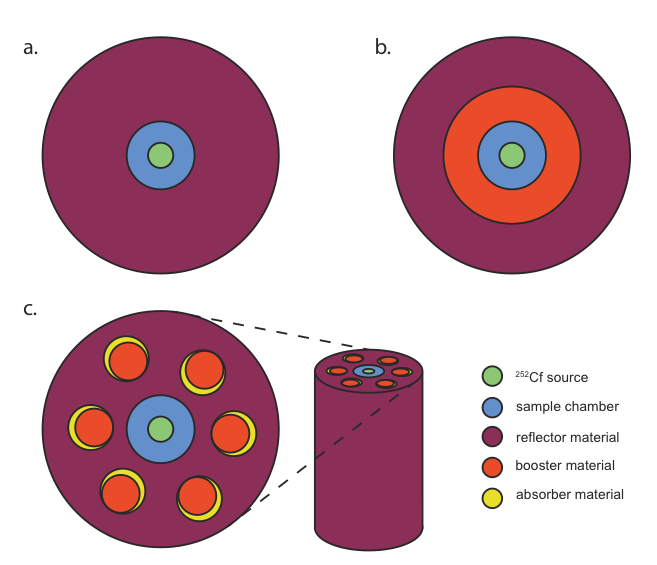
\includegraphics[width=0.5\textwidth]{Geometries.png}
  \caption{Configurations of devices for in-situ \ce{^{40}Ar}/\ce{^{39}Ar} geochronology. (a) A point source with a spherical shield/reflector, (b) a point source with spherical or cylindrical boosting material surrounded by a shield/reflector, (c) cylindrical assembly with centrally-located point source surrounded by boosting rods or rotatable boosting drums and shield/reflector.}
  \label{fig:geometries}
\end{figure}

To summarize, a neutron emitting device designed to irradiate samples for Ar/Ar geochronology applications will require three basic components: a neutron source, a sample chamber, and a shield. To optimize the transmutation of \ce{^{39}K} into \ce{^{39}Ar} and minimize competing reactions that may skew the age, the neutron source should provide a neutron flux with a large proportion of the flux in the fast energy range. The source strength should be around $10^{10}$ n/cm$^2$s or $10^{11}$ n/s to ensure that the sample does not require too long an irradiated time. Further, the neutron source should have some longevity (achieved with either a long half-life or a slow burnup) to ensure that the device can perform Ar/Ar geochronology for the length of the rover lifetime. The sample should not exceed 200\celsius\ during any time prior to step-heating, which can be prevented with either a source with a low power-density or a heat removal system. The rover should not receive a neutron flux from the source greater than $10^7$ n/cm$^2$s, which can be achieved with a shield. However, the entire system cannot exceed more than $\sim$70 kg, so the shield must be optimized to be of high absorption but low mass. It is the interplay between these parameters that significantly restricts the device design and makes this work novel. 

The subsequent subsections detail the design options analyzed for the device. Section \ref{sec:sources} elaborates on the various sources that could be used to supply neutrons for the device. This includes passive fission sources, or sources undergoing fission without an induced reaction; passive capture sources, or sources that supply neutrons by undergoing a capture of an alpha particle; and boosting materials, or materials that require a capture of a neutron to induce fission or produce neutrons. Section \ref{sec:shields} covers the shield material selection and geometric configurations that were considered for this application. Last, section \ref{sec:others} covers non-neutronic design details for Ar/Ar geochronology applications in addition to explaining the rationale behind the neutron sources that were not considered for this study. 

All neutron transport simulations were done using MCNP5~\cite{brown_mcnp_2002}. For design configurations using \ce{^{252}Cf}, a point source with watt fission energy spectrum was used. The total number of particles run in fixed-source problems varied, but were chosen such that any result had <2\% error. For criticality calculations (used for some boosting materials), the kcode card was used with 2,000 particles per generation, skipping 50 generations, and using 150 generations. For shielding calculations, the decrement in the flux was calculated with an f1 tally and angular binning to count the outgoing particles in each region of the shield.
%I don't know what the decrement in the flux means? Do you mean the outgoing flux to figure out the flux reduction?
 Last, reactions in non-critical boosting materials (Fig. \ref{fig:beboosters}) were calculated with an f4 tally and reaction rate multipliers.

\subsection{Neutron Source}
\label{sec:sources}

A number of neutron source options were considered for the neutron emitting device. Isotopes decaying by some probability of spontaneous fission offer a predictable neutron source flux with a sufficiently large proportion of fast neutrons. However, these sources also decay over time, so sample irradiation times will increase over the lifetime of the device to achieve a desired fluence. Passive capture sources, like ($\alpha$,n) reactions, are attractive because two elements are required to create neutrons. This could mean source strength could be user-controlled, prolonging the life of the neutron source and, consequently, the entire device. Boosting materials offer similar benefits to the latter and can be chosen to maximize fast neutron creation. 

The neutron source and booster have a few design constraints. First, the source must provide a fluence comparable to that of a terrestrial research reactor in $\sim$200 days or less. This fluence should be achievable throughout the lifetime of the device, meaning that the half-life should not be too short. Second, the neutron energy spectrum should be relatively fast to maximize the \ce{^{39}K}(n,p)\ce{^{39}Ar} reaction and minimize the competing Ar generating reactions. Third, the source should have a relatively low power density, to minimize the heat transferred to the sample chamber. Finally, the source should have a low mass to provide the required neutron supply. If the device can `shut down', then the shielding thickness for the source can be decreased as the device will have a lower passive dose rate during non-irradiation times. This decrease in shield thickness would allow for a greater proportion of the device mass to be dedicated to the neutron source. Depending on the feasibility of startup and shutdown of this device, this `low mass' could range between <1g to $\sim$30kg. 
% I think this is good, but I get the sense that some things are repeated quite a bit. I am on the fense about wanting to make it clear what is happening for which reason, and the desire to be concise. 

\subsubsection{Passive fission sources}

Table \ref{tab:fisssource} compares the total mass and heat output for a number of different spontaneous fission isotopes (SF BR is spontaneous fission branch ratio). This was calculated with existing fission yield data in the literature~\cite{england_evaluation_1995, axton_neutron_1985}.
No isotope seems to completely satisfy all of the requirements of the passive fission sources. Some have long half lives but require significant mass. Others create too much heat and will cause a premature release of natural and radiogenic argon. \ce{^{252}Cf} appears to most closely satisfy the heat output and mass requirements while also having a reasonably long half-life. \ce{^{252}Cf} has the added benefit of broad user experience \cite{martin_production_2000} and a slightly faster neutron energy spectrum than that of \ce{^{235}U} \cite{hjalmar_energy_1955}. However, using \ce{^{252}Cf} as the sole neutron source in the device does pose some disadvantages: the device lifetime is unlikely to exceed the lifetime of the Mars rover as several half-lives will pass during the course of a Martian mission, and it will take several years in a specialized reactor to produce enough \ce{^{252}Cf} to supply the source requirement desired for these purposes. This will take time and likely come at a large monetary cost. 

 \begin{table}
  \centering
  \caption{Passive neutron sources decaying by spontaneous fission}
  \begin{tabular}{l|ccccc}
    \toprule
    Source & Mass for $10^{11}$ $\frac{n}{s}$ & $\frac{n}{s-mg}$ & $t_{1/2}$ & SF BR (\%) & Heat Out ($\frac{Watts}{10^{11} src-n}$) \\
    \midrule
    \ce{^{252}Cf}& \num{43} mg & \num{2.3e9} & \num{2.645} y & \num{3.82} & \num{1.43} \\
    \ce{^{250}Cf} & \num{9.5} g & \num{1.1e10} & \num{13.08} y & \num{0.08} & \num{31}  \\
    \ce{^{248}Cm} & \num{2.1} kg & \num{4.7e10} & \num{3.5e5} y & \num{8.26} & \num{1.04}  \\
    \ce{^{246}Cm} & \num{9.8} kg & \num{1.0e10} & \num{4.7e3} y & \num{0.03} & \num{90}  \\
    \ce{^{244}Cm} & \num{9.8} kg & \num{1.0e10} & \num{18} y & \num{1.3e-4} & \num{2.4e4}  \\
    \ce{^{253}Es} & \num{274} g & \num{3.6e8} & \num{20} d & \num{8.7e-6} & \num{2.1e5}  \\
    \ce{^{254}Fm} & \num{0.2} mg & \num{5.0e11} & \num{3.24} h & \num{0.06} & \num{33}  \\
	\bottomrule
  \end{tabular}
  \label{tab:fisssource}
\end{table}

\subsubsection{Passive capture sources}

Passive capture sources \cite{weise_neutron_1984,jacobs_energy_1983,marsh_high_1995} are those that generate neutrons by an $\alpha$ capture reaction (neutron capture is detailed in a subsequent section). Originally, these sources were attractive because separation of the $\alpha$ emitter from the target would cease neutron production. The ability to `shut down' the neutron source would reduce the required neutron shielding for the Mars rover (assuming dose limits are fluence rather than dose-rate dependent) and only require that the rover is constantly shielded from $\alpha$ particles.  Additionally, the neutron energy spectrum from this reaction is relatively fast. However, the total neutron production is on the order of a few  neutrons per $10^6\:\alpha$ particles per second or less for most materials \cite{weise_neutron_1984,jacobs_energy_1983}. Consequently, for a $10^{11}$ neutron/s source, a roughly $10^{17}$ $\alpha$/s source would be required. To obtain an alpha source this large, it would either be of significant mass, which will violate mission limits, or with a short half-life, which will not meet time requirements. Furthermore, the ($\alpha$,n) source must be homogeneously mixed to optimize the neutron production rate, which would invalidate its original attractiveness of being able to shut down. While these sources have been proposed for passive Ar/Ar applications in the past~\cite{li_evaluation_2011}, the authors do not believe that this source can realistically provide the required neutrons for geochronology applications. 

\subsubsection{Boosting material}

The boosting materials considered loosely fall into two categories: induced fission neutron sources, and neutron capture neutron sources. Both of these sources require an additional driving neutron source to produce neutrons. Induced fission sources can offer substantial multiplicitave boosting if the device configuration is near critical.  Much of the previous work on determining the minimum critical mass of induced-fission sources  was done with homogenized layers with differing ratios of fissionable material and moderator to enhance thermally-induced fission neutrons \cite{karni_semi-automated_keff,karni_smores_2003,goluoglu_smoresnew_2002}. This is not an attractive option for this application since a large fraction of the neutron flux will be thermal and thus unusable for the \ce{^{39}K}(n,p)\ce{^{39}Ar} reaction. Of the induced fission sources, uranium and plutonium oxides (chosen for their chemical stability) were considered; their results are illustrated in Fig.\ \ref{fig:boosters}. This figure was produced with a geometry like that illustrated in Fig.\ \ref{fig:geometries}b, with fissionable boosters in a spherical shell around the sample chamber. Surrounding the fissionable material is a polyethylene shield/reflector. \ce{^{233}U}, \ce{^{241}Pu}, and \ce{^{239}Pu} are seen as the most attractive boosters because they require the lowest mass to approach criticality. This is due to to their higher epithermal fission cross sections, which eliminate the requirement for substantial moderation to approach a critical state. This also results in a faster neutron energy spectrum supplied to the sample chamber, which is optimal for this application. 

\begin{figure}
  \centering
  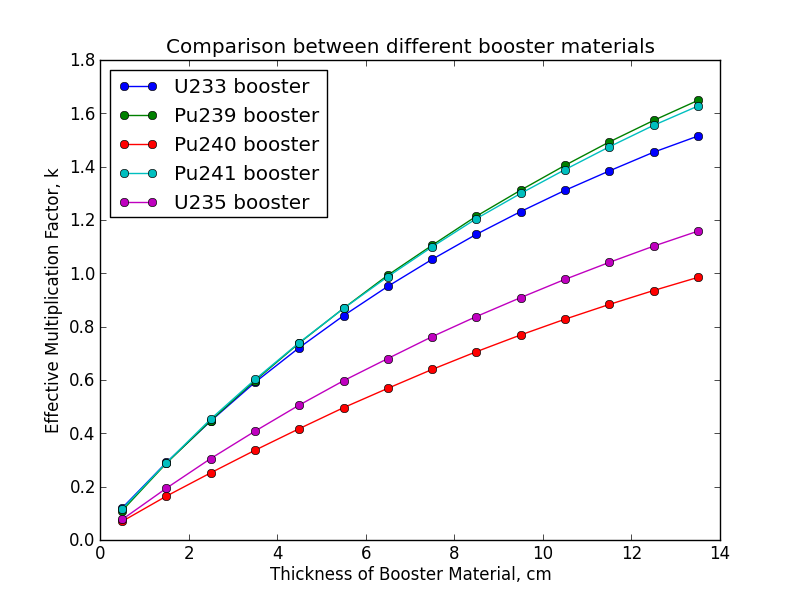
\includegraphics[width=4.5in]{Boosters.png}
  \caption{Induced fission neutron boosters}
  \label{fig:boosters}
\end{figure}

Of the neutron capture sources, the most attractive appeared to be the (n,2n) and (n,3n) fast neutron reactions in beryllium metal. A variant of Fig.\ \ref{fig:geometries}b was simulated with MCNP5 with a \ce{^{252}Cf} point source surrounded by a spherical shell of \ce{^{9}Be} metal shielded with Premadex, which is a hydrogenous material enriched in \ce{^{6}Li}.
% I'm not exactly sure what you're asking needs a citation. The geometries figure was produced Leah, but should I refer to the corporate website for Premadex? 
% Yep, I'm looking for a citation for Premadex :)
To find the best design, the thickness of the \ce{^{9}Be} shell was varied; Fig.\ \ref{fig:beboosters} summarizes these results. As the thickness of \ce{^{9}Be} increases so does the flux boost, peaking at a $\sim$10\% boost with an 8.5cm shell around the point source. Although this boost is not negligible, it is not worth the added mass of $\sim$5.6kg, which would only offset a short increment of \ce{^{252}Cf} decay losses. 

\begin{figure}
  \centering
  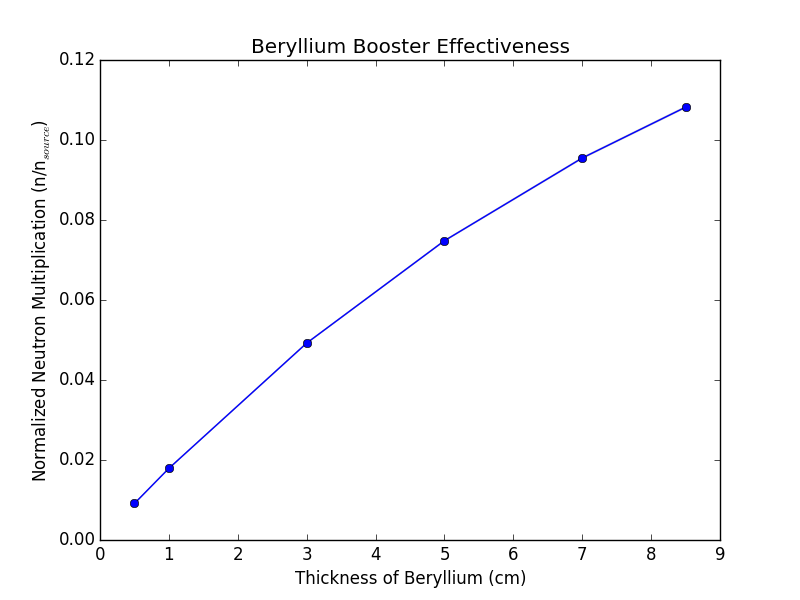
\includegraphics[width=4.5in]{Be_boost.png}
  \caption{Boosting the neutron flux with beryllium}
  \label{fig:beboosters}
\end{figure}
% Can you crop the edge lines out of this figure? It's the only one with them.

\subsection{Neutron Shield Design}
\label{sec:shields}

The most basic shield design is surrounding a point source of neutrons with a \ce{^{252}Cf} energy spectrum with a spherical shell of shield material. Figure \ref{fig:basics} illustrates the reduction in source strength as a function of radial distance from the point source for a number of shield material options.% (say what the materials you use are; I have no idea what the things in the legend are). %I'm updating these material names in my figure. It will look better soon
The materials comprised of light elements perform far better than the thermal neutron-absorbing metals, which is expected since without low atomic mass materials there is no moderator to slow neutrons to thermal energies where they will be absorbed. Of the two hydrogenous materials, Premadex appears to perform better at source reduction with shallow depths into the shield, and polyethylene appears to outperform with thicker shields. It should be noted that a substantial reduction in mass could be designed in the shield if the radial thickness is reduced. As these shields are spherical, the mass will increase with $r^3$, which directs device design towards thinner shields.  


\begin{figure}
  \centering
  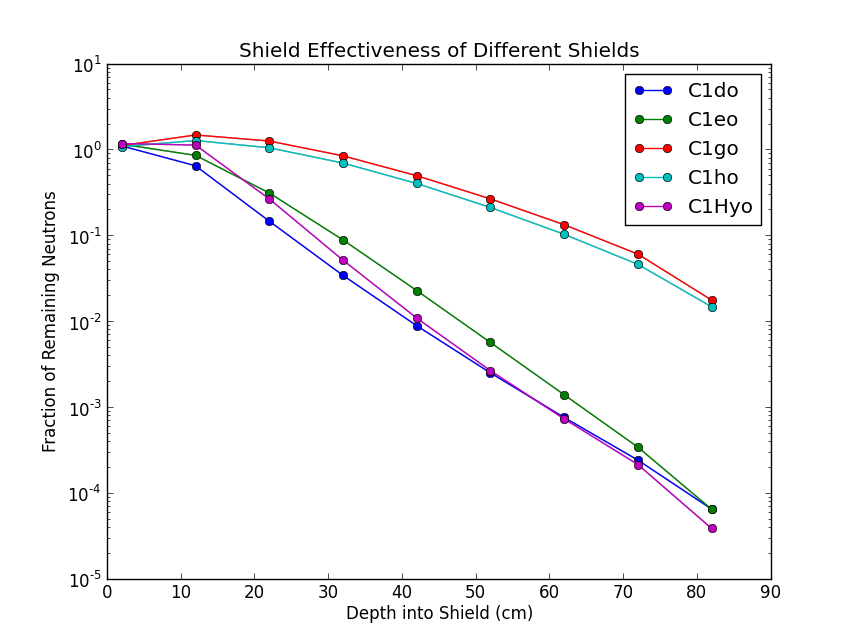
\includegraphics[width=4.5in]{Basics.png}
  \caption{Performance comparison for various shield material options}
  \label{fig:basics}
\end{figure}

Based on these observations, a composite shield designed to moderate and then absorb neutrons is likely the best option to reduce the radial thickness of required shield material. The materials with high thermal neutron absorption cross sections could rapidly reduce the radial shield thickness by removing large populations of thermal neutrons from the shield. This can be achieved by first moderating the fast fission neutrons from the \ce{^{252}Cf} source with a low atomic mass material. At the point in the moderating material at which there is no increase in thermal neutrons for an increase in moderator thickness, a foil of a strong thermal neutron absorber can be used to remove these neutrons. By alternating these materials, the flux can be removed in a shorter radial thickness than a single material alone. 

Figure \ref{fig:chars} compares the relative fraction of fast neutrons to thermal neutrons at various locations within a pure polyethylene or Premadex shield. The location at which the peak thermal flux occurs is an ideal candidate for foil placement. For polyethylene, Fig.\ \ref{fig:polychar} indicates that the maximum thermal neutron flux fraction occurs $\sim$15-20 cm away from the point source, where nearly 85\% of neutrons are thermalized. For Premadex, this location is at $\sim$12-15 cm (Fig.\ \ref{fig:premchar}), where about 47\% of neutrons are thermalized. This indicates that the foil placement could occur at a shallower depth into the Premadex shield, but it would likely remove fewer neutrons than a foil placed in the same location in the polyethylene shield. If a composite shield design is used for the device, polyethylene layered with either cadmium or gadolinium is the most attractive candidate. 


\begin{figure}
	\centering
	\begin{subfigure}{0.49\textwidth}
		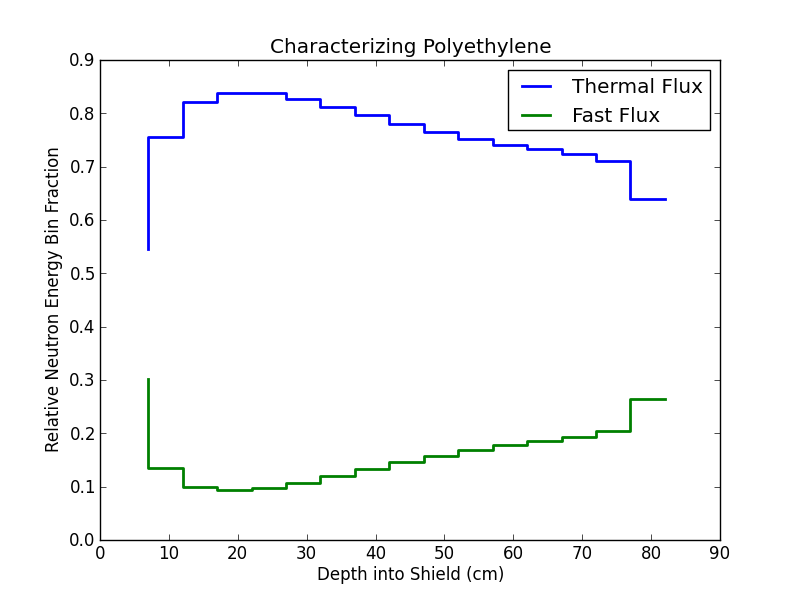
\includegraphics[width=\textwidth]{Poly_char.png}
		\caption{Polyethylene}
		\label{fig:polychar}
	\end{subfigure}
	\begin{subfigure}{0.49\textwidth}
		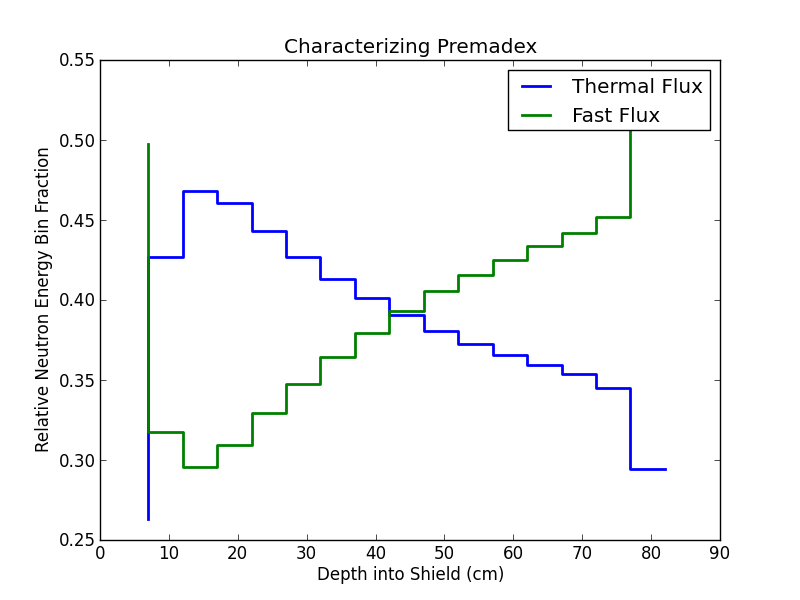
\includegraphics[width=\textwidth]{Prem_char.png}
		\caption{Premadex}
		\label{fig:premchar}
	\end{subfigure}
	\caption{Neutron energy spectra comparison between thermalizing shield options. Thermal energies are below 0.1eV and fast energies are greater than 0.1MeV.}
	\label{fig:chars}
\end{figure}

\subsection{Other Considerations}
\label{sec:others}

There are many additional considerations that will impact the source, sample holder, and shield design. A device optimized for the in-situ irradiation and age determination of geological samples requires an instrument payload in addition to the neutron emitting device. This will include, but is not limited to: a drilling mechanism, a mass spectrometer, and a system with which to heat up the sample to perform step-heating. These instruments, such as a mass spectrometer, can be optimized to have a greater abundance sensitivity. This could offset the loss of precision from a lower flux neutron source, but will undoubtedly come at a greater mass expense. Prioritizing which of these is more important will be imperative in moving forward with future designs. Including these components' contributions to the overall device mass will place an even greater limit on the neutron source and shielding masses. A more detailed consideration of each of these components and their mass will be in a forthcoming publication. For the purposes of this paper, the device including only the neutron source/booster and shielding contributed to the total device mass. 

The mass constraints on the mission could also change. The total mass threshold could be increased if the RTG on the rover could be replaced with the neutron device. This would require a much more sophisticated heat removal and power conversion system than we have proposed for the device described in this paper. Furthermore, the need of a small neutron emitting device could be avoided if other space reactor concepts are considered for future missions to Mars. In this case, a system not unlike the setup at the Oregon State TRIGA reactor could be designed for sample irradiation.
% you probably also need a reference for the oregon state triga reactor setup

Terrestrial Ar/Ar geochronology devices have much more flexibility in design than this passive source for Mars. The authors did not consider compact fusion sources, which have been considered for terrestrial \ce{^{40}Ar}/\ce{^{39}Ar} geochronology \cite{renne_application_2005}, as they are not mass-feasible for this application. Furthermore, we did not consider critical configurations of the device, as the device will be irradiating the sample for hundreds of days at a time and a system to compensate for reactivity feedback and other physical effects will add unnecessary complexity to  design criteria that are already highly constrained. Furthermore, low-mass critical devices are optimized to have significant moderation, which would not be ideal for this application. 

The shield analyzed in the previous sections did not consider activation effects or bubble formation from long-term neutron exposure to the shield. Both of these effects could augment the effectiveness of the shield over time. In particular, foils in the composite shield may lose effectiveness early on in the mission due to its high absorption cross section. The foils would then supply more radiation damage to the rover--from activation-produced photons--than protection, invalidating their use as a shield. The structural integrity of the shield could also be compromised because of long-term neutron exposure, which was also not considered here.  


%%%%%%%%%%%%%%%%%%%%%%%%%%%%%%%%%%%%%%%%%%%%%%%%%%%%%%%%%%%%%%%%%%%%%
\section{Feasibility of Device Configurations}
\label{sec:feasibility}

The neutron emitting device for remote, passive, Ar/Ar geochronology must at minimum be comprised of a neutron source, sample chamber, and shield. Several material options and geometric configurations have been proposed in the preceding pages to constitute such a device. Each option varies in its benefits and drawbacks; a successful design will find a compromise that satisfies each of the requirements for the device. Here the feasibility of each option is presented and analyzed. A preliminary design that most satisfactorily achieves each requirement will be proposed. 

The neutron sources considered were designed to provide a variety of options in constructing the device. Many elements decaying by spontaneous fission can be obtained that supply the required source strength of $\sim10^{11}$ n/s. However, \ce{^{252}Cf} appears to be the best candidate; it satisfies the requirements of having a low power density, low mass, adequate half-life, and has a broad user experience. Alternatively, $\alpha,n$ neutron sources do not appear attractive as they will require either a short half-life or significant mass to achieve the desired flux objective. %Of the proposed neutron sources, \ce{^{252}Cf} is the best overall candidate. 

Boosting material offers enhanced neutron production with the possible benefit of a removable source, which would lower the basal neutron dose rate to the rover and result in reduced shielding requirements. This would be of enormous benefit to the device, as a $10^{11}$ n/s point source of \ce{^{252}Cf} would require a substantial quantity of shielding to decrease the flux to the rover to $10^{7}$ n/cm$^2$s. Of the boosting materials considered, the (n,2n) and (n,3n) reactions in beryllium proved to have the least benefit, adding $\sim$10\% boost with a 5.3kg additional mass. The fissionable boosters, if constructed in a near-critical state, offer substantially more boosting benefit. However, even the boosters with the highest multiplicity (\ce{^{233}U}, \ce{^{239}Pu}, \ce{^{241}Pu}) required $\sim$20kg of material to approach criticality. This at first may seem attractive, but adding 20cm of polyethylene shielding to this spherical design would add $\sim$80-90kg of mass, moving this design out of the realm of feasibility. Further, these simulations were performed with a 4$\pi$ polyethylene reflector surrounding each booster. If no shield/reflector were used, the critical mass requirement would be higher, as fewer thermal and epithermal neutrons would exist to induce fission reactions.

The shield materials will comprise the largest fraction of the mass of the device. Placing the source 50cm away from the rover electronics will reduce the flux to $3 \times 10^6$ n/cm$^2$s, which is acceptable but still very close to the limit of the CCD cameras. Adding a 30cm spherical shell of polyethylene to this will reduce the flux by an additional $\sim$97\%. The total payload for this particular configuration (120kg) far exceeds the mass limitation for instrumentation of the rover.  Adding a foil of cadmium or gadolinium to the shield will reduce the flux substantially with a very small linear distance. This can be used to decrease the thickness , and thus the mass, of the shield.

It appears that elimination is the path towards a device design. 
% I don't know what this sentence means?
The most optimal neutron source is a \ce{^{252}Cf} source with no boosting material. Because the \ce{^{252}Cf} source is of such low mass, a significant proportion of the device mass can be dedicated to the shield. As it stands, even a spherical polyethylene shield will exceed the $\sim$70kg mass limitation of the device. Instead, we propose shielding only the fraction of the \ce{^{252}Cf} solid angle containing the rover, and not dedicating as much shielding to the planetary surface of mars. If only 10\% of the 4$\pi$ point source is shielded with polyethylene, the total device mass is $\sim$12kg. This is satisfactory for the objectives that were proposed in earlier sections and leaves an adequate mass allotment for other Ar/Ar instrumentation.

The device proposed in this paper is preliminary, and a great amount of analysis will be required for a more complete design. Selecting a mass spectrometer will provide a more concrete figure for the neutron source strength or flux. Performing heat transfer calculations to ensure that the sample chamber does not exceed 200\celsius\  will also be necessary. The shielding analysis should also include photons in future designs to ensure that the overall dose rate to the rover is not unacceptable. Further, selecting a power source to provide sufficient energy with which to step heat the sample to acceptable temperatures will be important since both \ce{^{40}Ar}/\ce{^{39}Ar} and \ce{^{40}K}/\ce{^{40}Ar} age calculations may be skewed without adequate heating. The most recent K/Ar age sample from Mars was heated to 890\celsius \cite{farley_situ_2014}, which does not reach the temperatures usually required for complete sample step heating, $\sim$1200\celsius \cite{mcdougall_geochronology_1999}. Powering a device to heat the sample to this temperature may temporarily disable the rover or even exceed current design limitations.

%%%%%%%%%%%%%%%%%%%%%%%%%%%%%%%%%%%%%%%%%%%%%%%%%%%%%%%%%%%%%%%%%%%%%
%\section{Future Work}
%\label{sec:future}
% If you end up being tight on space, you can cut down this section to just briefly say that you need to consider other things. You could make it just one paragraph in conclusions.
%Thus far, the neutronic feasibility of this device design has been explored. However, a number of other considerations must also be accounted for in greater detail in future analyses. Heat transfer calculations should be performed to ensure that the sample temperature will not exceed 200\celsius, which would lead to premature release of trapped argon in the sample. This calculation is contingent upon concrete knowledge of the design materials and geometry, and could be performed with some finite element heat transfer package. 
%
%Furthermore, selecting a power source to provide sufficient energy with which to step heat the sample to acceptable temperatures will be important since both \ce{^{40}Ar}/\ce{^{39}Ar} and \ce{^{40}K}/\ce{^{40}Ar} age calculations may be skewed without adequate heating. The most recent K/Ar age sample from Mars was heated to 890\celsius \cite{farley_situ_2014}, which does not reach the temperatures usually required for complete sample step heating, $\sim$1200\celsius \cite{mcdougall_geochronology_1999}. Powering a device to heat the sample to this temperature may temporarily disable the rover or even exceed current design limitations. 
%
%The shielding analysis and optimization detailed in this paper was exclusively for neutron shielding. Future rovers will also have photon dose limits, which will require shielding to ensure that the electronics do not degrade at an unacceptable rate. The addition of thermal neutron absorbers in a composite shield option, like Cd or Gd, will produce high energy photons that may have adverse effects on the overall damage rate of the device. Further optimization to minimize shield mass and volume more explicitly will be beneficial. Should fissionable booster options be considered, it would also be ideal to minimize the boosting material mass to achieve the desired subcritical multiplication factor. %Existing software to determine the minimize critical mass \cite{goluoglu_smoresnew_2002,karni_semi-automated_keff,karni_smores_2003} of systems and optimize shield designs \cite{greenspan_material_1994,greenspan_swans:_2001} are available in the SCALE package \cite{bowman_scale_2003}. Using this software in future design iterations would aid in the convergence to a realistic device design.  
%
%%%%%%%%%%%%%%%%%%%%%%%%%%%%%%%%%%%%%%%%%%%%%%%%%%%%%%%%%%%%%%%%%%%%%
\section{Conclusions}
\label{sec:conclusions}

A compact neutron source is an attractive candidate to induce the necessary reactions for  \ce{^{40}Ar}/\ce{^{39}Ar}  geochronological applications on future, unmanned, missions to extra-terrestrial bodies where sample return is neither feasible nor likely. However, the vast range of overall dose and dose rate limits for existing rover designs lead to ambiguity in shielding designs, making optimization difficult. In this paper we examine a variety of sources, boosters, and shielding materials to provide suggestions for the best candidates for a final design.

Some major challenges are longevity of the source and reducing shielding mass. The  exclusive use of a \ce{^{252}Cf} fission neutron source challenges source lifetime requirements. The lifetime could be extended with boosting material, but that would require moderation of all 4$\pi$ solid angles of the boosting material to achieve increased efficiency in neutron-induced fission. The addition of both shielding material and enough boosting material to achieve a high enough effective multiplication factor renders this configuration likely unfeasible. We therefore recommend using \ce{^{252}Cf} without a booster. Shielding can be reduced over most solid angles of the point source rf extreme dose rates to the martian surface are acceptable. Then, only the solid angle containing the rover requires shielding. 

Although it appears that there cannot be a `perfect' device designed for Ar/Ar applications, there are variants of the device that will satisfy the requirements detailed in earlier sections. 
% describe configuration: Cf point source with poly shield and film absorber layers.
This configuration produces a device that has: low mass, adequate flux with a substantial fraction of fast neutrons, low thermal insulation, sufficient rover shielding, and will last several years. As the design has only a spontaneous fission neutron source, this device does have issues with longevity, and Ar/Ar geochronology will undoubtedly be difficult and have low precision towards the end of the rover's lifetime. However, this device is the most feasible given the restrictions imposed for martian Ar/Ar geochronological applications. 
 
 

%%%%%%%%%%%%%%%%%%%%%%%%%%%%%%%%%%%%%%%%%%%%%%%%%%%%%%%%%%%%%%%%%%%%%
\section{Acknowledgments}

The primary authors would like to thank their collaborators for their wealth of knowledge and support on this project. In particular, we would like to thank the participants of our design review, held in Spring of 2014: Paul Renne, Tim Becker, Karl Van Bibber, Peter Hosemann, Max Fratoni, Rachel Slaybaugh, Richard Firestone, and Cory Waltz. We also would like to thank the European Space Agency for their generous financial support for this endeavor. Additionally, we thank Roger Scott, David Gilliam from NIST, David Thomas from NPL, and Ken Farley for their valuable advice and input on this project. 

%%%%%%%%%%%%%%%%%%%%%%%%%%%%%%%%%%%%%%%%%%%%%%%%%%%%%%%%%%%%%%%%%%%%%
\setlength{\baselineskip}{12pt}

\bibliographystyle{mc2015}
\bibliography{references}

%%%%%%%%%%%%%%%%%%%%%%%%%%%%%%%%%%%%%%%%%%%%%%%%%%%%%%%%%%%%%%%%%%%%%

\end{document}
